\documentclass[aspectratio=169]{beamer}
% INCLUDE beamerthemeMumbai.sty
\usetheme[
    infolines-footline,
    miniframes={subsection=false} ]{Mumbai}

\usepackage{graphicx}
\usepackage{xcolor}
\usepackage{colortbl}
\usepackage{hyperref}
\usepackage[many]{tcolorbox}
\usepackage{qrcode}
\usepackage{minted}
\usepackage{graphicx}

%Information to be included in the title page:
\title{Efficient Estimation of Word Representations in Vector Space}
\author{Ivan N., Ryan L., Chaitanya M.}

\usetheme{default}
\institute{UC Riverside}
\date{January 23, 2024}

\begin{document}

\begin{frame}
\titlepage
\end{frame}

\section{Background}
\begin{frame}[fragile]
\frametitle{Background}

What is a word vector?

\begin{minted}{cpp}
vectorize("hello") -> [0, 0.23, 0, .10, 0.5, 0.75, ...]
\end{minted}


\vskip 0.2in

Problem(s):
\begin{itemize}
    \item Current methods \textbf{do not truly capture similarity} between words.
    \item Computational capabilities only allow for \textbf{limited size} of data.
    \item In-domain data is limited.
\end{itemize}

\end{frame}

\begin{frame}
\frametitle{Background}
Goal(s) of the Paper:
\begin{itemize}
    \item Capture similarity between words in a better way.
    \item More efficiently compute word vectors.
    \item Test performance of this model.
\end{itemize}

\end{frame}

\section{Methodology}
\begin{frame}
\frametitle{Methodology}

\begin{columns}

\begin{column}{0.5\textwidth}
    Two proposed methods:

    \vskip 0.5in

    \begin{itemize}
        \item[1.] Continuous Bag-of-Words Model
        \item[2.] Continuous Skip-gram Model 
    \end{itemize}
\end{column}

\begin{column}{0.5\textwidth}

\begin{center}
    \textbf{Continuous Bag-of-Words}
\end{center}

% insert image
\begin{center}
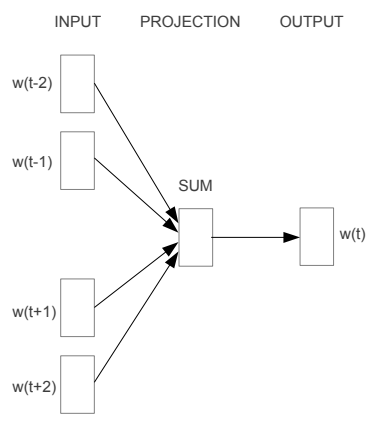
\includegraphics[scale=0.35]{cbow.png}
\end{center}

\begin{itemize}
    \item Complexity: $Q = N \times D + D \times log_2(V)$ % Q = N × D + D × log2(V )
\end{itemize}

\end{column}

\end{columns}

\end{frame}


\begin{frame}
\frametitle{Methodology}

\begin{columns}

\begin{column}{0.5\textwidth}
    Two proposed methods:

    \vskip 0.5in

    \begin{itemize}
        \item[1.] Continuous Bag-of-Words Model
        \item[2.] Continuous Skip-gram Model 
    \end{itemize}
\end{column}

\begin{column}{0.5\textwidth}

\begin{center}
    \textbf{Continuous Skip-Gram}
\end{center}

\begin{center}
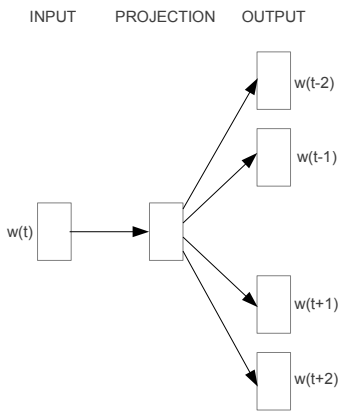
\includegraphics[scale=0.35]{csg.png}
\end{center}

\begin{itemize}
    \item Complexity: $Q = C \times (D + D \times log_2(V))$ % Q = C × (D + D × log2(V ))
\end{itemize}

\end{column}

\end{columns}

\end{frame}

\begin{frame}
\frametitle{Methodology}

Both of these models are considered Word2Vec

\begin{columns}
\begin{column}{0.5\textwidth}

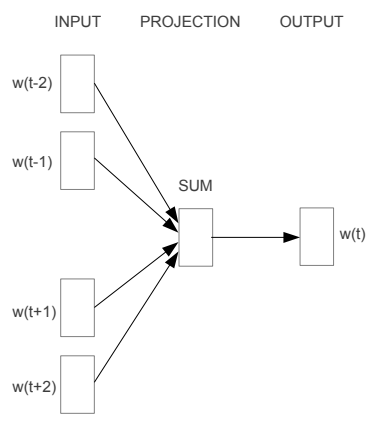
\includegraphics[scale=0.45]{cbow.png}

\end{column}

\begin{column}{0.5\textwidth}
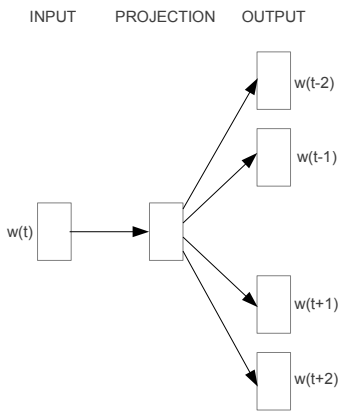
\includegraphics[scale=0.45]{csg.png}
\end{column}

\end{columns}

\end{frame}


\section{Results}
\begin{frame}
\frametitle{Results}

Summarized Results
\begin{itemize}
    \item Improved performance over other state-of-the-art methods for capturing word relationship information.
    \item A much more efficient method for generating word vectors.
\end{itemize}

\begin{center}
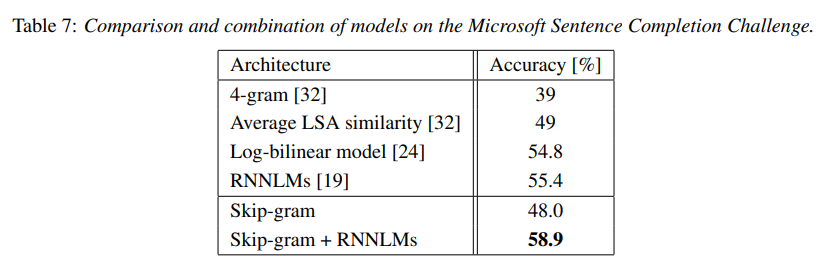
\includegraphics[scale=0.5]{microsoft.png}
\end{center}

\end{frame}

\begin{frame}
\frametitle{Results}

\begin{center}
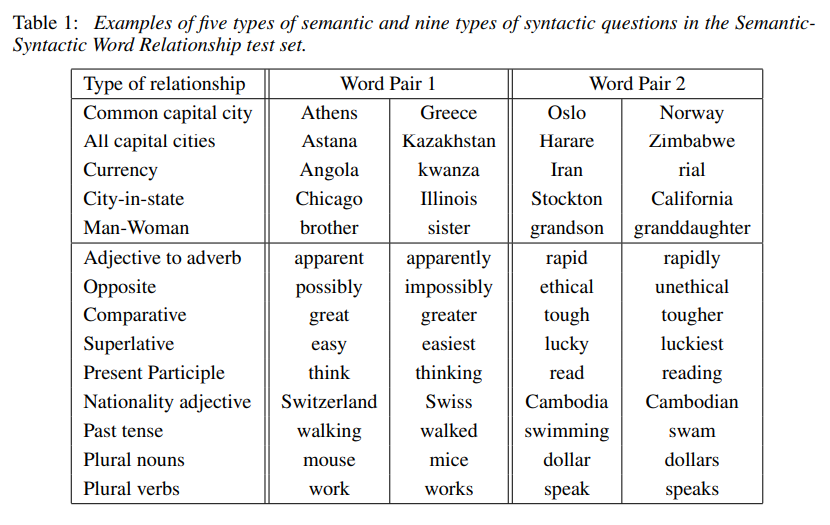
\includegraphics[scale=0.5]{speed.png}
\end{center}

\end{frame}

\begin{frame}
\frametitle{Results}

\begin{center}
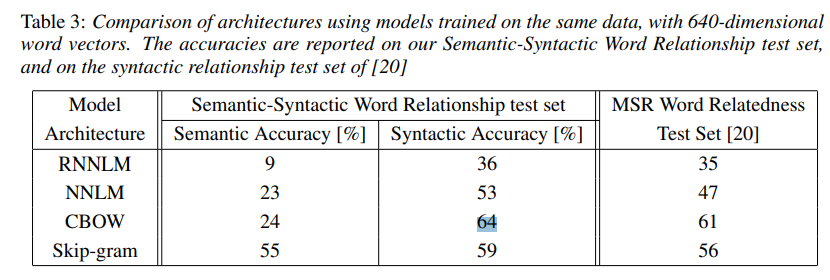
\includegraphics[scale=0.5]{results.png}
\end{center}

\end{frame}

\begin{frame}
\begin{center}

That's it! Any questions?

\end{center}
\end{frame}

\section{References}
\begin{frame}{References}
\frametitle{References}

\begin{itemize}
\item[1.] Mikolov, Tomas, et al. "Efficient estimation of word representations in vector space." arXiv preprint arXiv:1301.3781 (2013).
\item[2.] T. Mikolov, W.T. Yih, G. Zweig. Linguistic Regularities in Continuous Space Word Representations. NAACL HLT 2013.
\item[3.] G. Zweig, C.J.C. Burges. The Microsoft Research Sentence Completion Challenge, Microsoft
Research Technical Report MSR-TR-2011-129, 2011.
\end{itemize}
\end{frame}

\end{document}